\documentclass[12pt]{article}

%Uporabljeni paketi
\usepackage[utf8]{inputenc}
\usepackage{cmap}
\usepackage{type1ec}
\usepackage[T1]{fontenc}
\usepackage{fancyhdr}
\usepackage{graphicx,epsfig}
\usepackage[slovene]{babel}
\usepackage{cite}

\usepackage[pdftex,colorlinks,citecolor=black,filecolor=black,linkcolor=black,urlcolor=black,pagebackref]{hyperref}
\usepackage{tikz}

%Velikost strani - dvostransko
\oddsidemargin 1.4cm
\evensidemargin 0.35cm
\textwidth 14cm
\topmargin 0.26cm
\headheight 0.6cm
\headsep 1.5cm
\textheight 20cm

%Nastavitev glave in repa strani
\pagestyle{fancy}
\fancyhead{}
\renewcommand{\sectionmark}[1]{\markright{\textsf{\thesection\  #1}}{}}
%\fancyhead[RE]{\leftmark}
\fancyhead[LO]{\rightmark}
%\fancyhead[LE,RO]{\thepage}
\fancyfoot{}
\renewcommand{\headrulewidth}{0.0pt}
\renewcommand{\footrulewidth}{0.0pt}
\graphicspath{ {images/} }

\newcommand{\gnuplot}{\textbf{gnuplot}}
\newcommand{\pgfname}{\textsc{pgf}}
\newcommand{\tikzname}{Ti\emph{k}Z}

\begin{document}
\setcounter{page}{1}
\pagenumbering{arabic}

\title{Bitcoin Block Withholding Attack : Analiza in ublažitev napada}
\author{Anej Budihna,Luka Golinar, Matjaz Glumac}


\maketitle
\begin{abstract}

Avtorji se posvetijo dvema problemoma: prvi je študija različice napada imenovanega "bločno prikrivanje" (angl. block withholding attack - BWA) v Bitcoinih in drugi je priporočilo rešitev za preprečitev vseh obstoječih vrst  BWA napadov. Predstavijo analize strategij sebičnega Bitcoin rudarja, ki v potuhi z neko skupino rudarjev poskuša napadati neko drugo skupino in pri tem dobi določeno nagrado, ker je prisostvoval pri napadu na drugo skupino. Tak napad so avtorji poimenovali "sponzorirani napad z bločnim prikrivanjem". Poleg tega predstavijo podrobno kvantitivno analizo dobičkonosnosti, ki jo lahko sebični rudar pridobi s tem, ko rudar uporablja omenjen napad v različnih primerih. V članku avtorji dokažejo, da ob določenih pogojih lahko napadalec optimalno poveča svoj prihodek z uporabo nekaterih strategij in s pametnim izkoriščanjem svojih računalniških virov. Pokažejo tudi, da lahko napadalec uporabi to strategijo za napad na obe skupini, da bi pri tem lahko dosegel višjo dobičkonosnost.
\indent Najpomembneje, predstavijo strategijo, ki se lahko učinkotivto zoperstavi napadu bločnega prikrivanja v katerikoli rudarski skupini. Prvo priporočajo generično shemo, ki uporablja kriptografsko zavezujoče sheme za zoperstavitvi takemu napadu. Nato priporočajo alternativno implementacijo enake sheme z uporabo razpršilnih (angl. hash) funkcij. Taka shema ščiti skupino rudarjev pred zlonamernimi rudarji, tako navadnimi kot tudi administratorskimi redarji. Tako ta shema kot tudi druge njene različice ponujajo obrambo pred BWH napadi s tem, da onemogočijo možnost, da rudarji razlikujejo med celovitimi in delnimi dokazi dela. Prav tako pa te sheme omogočajo zaščito, da administratorji ni omogočeno goljufanje znotraj skupine katero nadzorujejo. Shemo se lahko implementira tako, da se napravi korenito spremembo na obstoječem Bitcoin protokolu.
Na koncu se tudi posvetijo analizi varnosti opisane sheme.

\end{abstract}
{\large \bf Ključne besede:} Bitcoin rudarjenje, napad z bločnim prikrivanjem, sebičen rudar, rudarske skupine, zavezujoče sheme.

\section{Uvod}
Bitcoin je popularna kripto valuta, ki jo je prvo priporočil Satoshi Nakamoto \cite{nakamoto} leta 2008. Transakcije so javno preverljive v glavnem računu imenovanem "bločna veriga" (angl. blockchain). Bločna veriga je sestavljena iz veliko blokov, ki potrdi različne transakcije. Uporabniki, ki ustvarjajo in preverjajo te bloke se imenujejo rudarji. Rudarji nato kot motivacijo pridobijo novo ustvarjene Bitcoin-e. Da bi se reguliralo pretok Bitcoinov se bloki ustvarijo približno vsakih 10 minut. Rudarji morajo rešiti uganko (kot dokaz dela - angl. proof of work (PoW)), če hočejo pridobiti spodbudne Bitcoin-e. Čeprav obstajajo alternativne valute kot Permacoin \cite{permacoin} in Retriecoin \cite{retriecoin}, ki uporabljajo shrambe namesto računanja za ustvarjanje valute, je dokazovanje dela, ki ga uporablja Bitcoin zaenkrat še vedno najboljši načrt. V \cite{economicsofbitcoin} so Kroll  in drugi pokazali, da Bitcoin rudarjenje ni tako "končno", vodeno z vlogami in motivacijsko kompatibilen sistem kot pravijo nekateri njegovi zagovorniki. Napadi z bločnim prikrivanjem \cite{analysisofbitcoin},\cite{financialcryptography}

\newpage

\section{Luka - page 5 and forth}


\begin{center}
  \begin{tabular}{ | c | c | c | c | c | }
    \hline
    $\alpha$ & $\beta$ & $\gamma$ & p' & $\bigtriangleup G_h^O $  \\ \hline
    0.200000 & 0.500000 & 0.700000 & 0.340000 & 0.248016 \\ \hline
    0.100000 & 0.900000 & 0.700000 & 0.400000 & 0.417396 \\ \hline
    0.200000 & 0.400000 & 0.700000 & 0.340000 & 0.214171 \\ \hline
    0.160000 & 0.600000 & 0.700000 & 0.330000 & 0.254052 \\ \hline
    0.200000 & 0.800000 & 0.700000 & 0.400000 & 0.394558 \\ \hline
    0.200000 & 0.900000 & 0.700000 & 0.400000 & 0.408747 \\ \hline
    0.200000 & 0.960000 & 0.700000 & 0.400000 & 0.414236 \\ \hline
    0.200000 & 0.990000 & 0.700000 & 0.400000 & 0.416150 \\ \hline
    0.200000 & 0.700000 & 0.700000 & 0.400000 & 0.415573 \\ \hline
  \end{tabular}
\end{center}
TABELA II: Tabelarični prikaz vrednosti $\bigtriangleup G_h^O $ za različne vrednosti ustreznih parametrov. $\alpha$ prikazuje računsko moč napadalca. $\beta$ prikazuje del računske moči, ki jo napadalec uporabi pri napadu na bazen rudarjev P. $\gamma$ prikazuje del spodbude, ki jo bazen P' pridobi zaradi napada napdalaca, ter jo z njim deli. p' predstavlja računsko moč P'.
\newline
\newline
Ker je 1 - $\alpha\beta$ dobiček P naraste $\frac{p'}{ 1 - \alpha\beta}$.  Torej je narastek dobička bazena rudarjev P'  $\frac{p'}{1 - \alpha\beta}$ - p' = $\frac{\alpha\beta p'}{1 - \alpha\beta}$
\newline

Sedaj je potrebno izračunati spodbudo A. Ker A za napad na P uporablja $\alpha\beta$ del svoje računske moči, lahko predpostavimo, da je računska moč aktivnega omrežja enaka 1 - $\alpha\beta$. Tukaj avtorji predpostavijo\cite{originalarticle}, da so vsi ostali rudarji v baznu P in P' pošteni. Spodbuda A je trojna. Najprej predpostavimo, da je dobiček A zasebnega rudarjenja enaka $ G_1 = \frac{\alpha(1 - \beta)}{ 1 - \alpha\beta}$. Pričakujoč delež spodbude rudarjenja v bazenu P je $ G_2 = \frac{p - \alpha\beta)}{ 1 - \alpha\beta} \frac{\alpha\beta}{p}$. Ponovno je potrebno izpostaviti, da je spodbuda pridobljena iz rudarjenja v bazenu P' zaradi napada na konkurenčni bazen (P) definirana z $ G_3 = G_P' * \gamma = \frac{\alpha\beta p' \gamma}{1 - \alpha\beta} $. 

Torej je skupen dobiček napadalca enaka:
\newline
\begin{equation} \label{eq:2}
G = G_1 + G_2 + G_3 = \frac{\alpha(p-\alpha\beta^2 + p'\beta\gamma)}{p(1 - \alpha\beta)}.
\end{equation}

\textbf{Iz zgornje enačbe so avtorji opazili, da se spodbuda napadalca večka, če napade večji bazen rudarjev, ter dobi spodbudo iz manjšega bazena rudarjev.}
\newline
Avtorji izpostavljajo, da je ko je napadalec uporabil le klasični BWH napad brez tajnega sporazuma z bazenom rudarjev P' je bil pričakovan dobiček enak: $ G = G_1 + G_2 + G_3 = \frac{\alpha(p-\alpha\beta^2 + p'\beta\gamma)}{p(1 - \alpha\beta)}. $ Naraščaj dobičeka, ki ga napadalec pridobi v razmerju z dobičkom originalnega BMH napada se izrazi z:
\newline
\begin{equation} \label{eq:3}
\bigtriangleup G_{BWH}^O = \frac{G}{G'} - 1 = \frac{p'\beta\gamma}{p - \alpha\beta^2}.
\end{equation}

Ker je $ \alpha\beta < p $ je torej $ \alpha\beta^2 < \alpha\beta < p $. Torej avtorji predpostavijo, da je $ \bigtriangleup G_{BWH}^O > 0.$ V primeru, da je bil napadalec pošten rudar je spodbuda, ki jo je precej iz poštenega rudarjenja enaka $G_h = \alpha$. Razmerje spodbude, ki jo napdalec sedaj prejme od tretjih blokov z NPB napadom se izrazi z $\bigtriangleup G_O^h = \frac{G}{G_h} - 1 = \frac{\alpha\beta p + p' \beta\gamma - \alpha\beta^2}{p(1 - \alpha\beta)}$. Če zamenjamo p z $ 1 - p' - \alpha - \alpha\beta$ dobimo,
\begin{equation} \label{eq:4}
\bigtriangleup G_O^h = \frac{G}{G_h} - 1 = \frac{\alpha\beta 1 - p' - \alpha - \alpha\beta + p' \beta\gamma - \alpha\beta^2}{(1 - p' - \alpha - \alpha\beta)(1 - \alpha\beta)}.
\end{equation}
\newline
\begin{figure}
  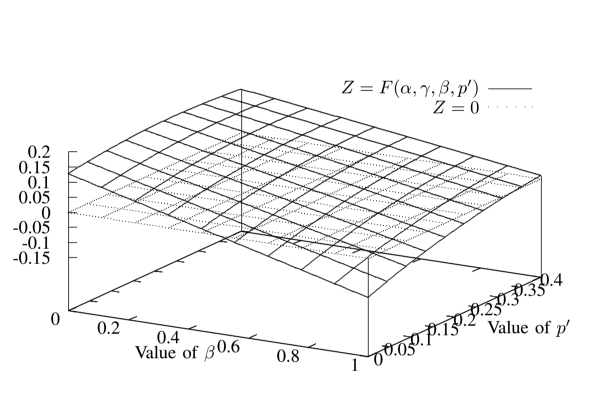
\includegraphics[scale=0.5]{image1.png}
  \caption{Grafični prikaz obnašanja $Z = F(\alpha, \gamma, \beta, p')$, ko sta $\alpha = 0.2, \gamma = 0.7$}
  \label{fig:boat1}
\end{figure}
\newline
\textbf{Izrek 1}. Naj bo $ \beta_0 \in (0, 1) $ tak, da je skupen dobiček napadalca enak $G|_\beta=\beta_0 = max(G|_\beta=\beta_0'): \forall\beta' \in [0,1]$. V tem primeru $\beta_0$ zadosti
\begin{equation}
A \beta_0^2 + B\beta_0 + C = 0
\end{equation}
kjer je $A = -\alpha^2(1 - \gamma)p', B = 4\alpha^2 - 2\alpha^3 - 2\alpha^2p' + 2\alpha p' - 2\alpha, C = \alpha^3 - 2\alpha^2 + 2\alpha^2 p' - 2\alpha p' - \alpha\gamma p' + \alpha + \alpha p'^2 - \gamma p'^2 + \gamma p' $.

\textit{Dokaz.} Dokazali smo, da je v trenutni nastavitvi skupni dobiček napadalca A enak $G = \frac{\alpha(p - \alpha\beta^2 + p'\beta\gamma)}{p(1 - \alpha\beta)}$. V primeru, da p zamenjamo z 1 - p' - $\alpha + \alpha\beta$ v Enačbi(2), dobimo skupni dobiček definiran kot:

\begin{equation}
G = \frac{\alpha(1 - p' - \alpha + \alpha\beta - \alpha\beta^2 + p' \beta\gamma)}{1 - p' - \alpha + \alpha\beta(1 - \alpha\beta)}
\end{equation}

Če diferenciramo po $\beta$, dobimo
$\frac{\partial G}{\partial\beta} = \frac{\alpha(-2\alpha\beta + \gamma p' + \alpha)}{(1 - \alpha\beta)(\alpha\beta - p' - \alpha + 1)} + \frac{\alpha^2(-\alpha\beta^2 + \gamma p'\beta + \alpha\beta - p' - \alpha + 1)}{(1 - \alpha\beta)^2(\alpha\beta - p' - \alpha + 1)} - \frac{\alpha(-\alpha\beta^2 + \gamma p'\beta + \alpha\beta - p' - \alpha + 1)}{(1 - \alpha\beta)(\alpha\beta - p' - \alpha + 1)^2}$. Avtorji so izraz poenostavili, ter dobili $\frac{\partial G}{\partial\beta} = \frac{Num}{Den}$, kjer sta, 
\newline
$Den = (1 - \alpha\beta)^2(1 - p' - \alpha + \alpha\beta)^2$
\newline
$Num = -\alpha^3(1 - \gamma)p'\beta^2 + (4\alpha^3 - 2 \alpha^4 - 2\alpha^3 p' + 2\alpha^2 p' - 2\alpha^2)\beta + (\alpha^4 - 2\alpha^3 + 2\alpha^3 p' - 2\alpha^2 p' - alpha^2\gamma p' + \alpha^2 + \alpha^2 p'^2 - \alpha\gamma p'^2 + \alpha\gamma p')$.
\newline
\newline
Opazimo lahko, da $Den \not= 0 \forall\beta \in [0, 1].$ Če se G razširi nad $\beta = \beta_0, \frac{\partial G}{\partial\beta}|_\beta=\beta_0 = 0$. Torej $-\alpha^3(1-\gamma)p' \beta_0^2 + (4\alpha^3 - 2\alpha^4 - 2\alpha^3 p' + 2\alpha^2 p' - 2\alpha^2)\beta_0 + (\alpha^4 - 2\alpha^3 + 2\alpha^3 p' - 2\alpha^2 p' - \alpha^2 \gamma p' + \alpha^2 + \alpha^2 p'^2 - \alpha\gamma p'^2 + \alpha\gamma p') = 0$. Zaradi tega, ker $\alpha \not= 0$, lahko izraz napišemo kot $-\alpha^2(1 - \gamma)p' \beta^2 + (4\alpha^2 - qalpha\gamma p' + \alpha + \alpha p'^2 - \gamma p'^2 - \gamma p'^2 + \gamma p') = 0$. 

\textbf{Lema 2.} Naj bo $ F(\alpha, \gamma, \beta, p') = A\beta^2 + B\beta + C $. V tem primeru je F(.) padajoča funkcija nad $ \beta $, če je $ \alpha $ manjše od 0.25.

\newpage
\begin{thebibliography}{9}
 
 \bibitem{nakamoto}
 S. Nakamoto, 
 \textit{Bitcoin: A peer-to-peer electronic cash system}, 2008.
 
 \bibitem{permacoin}
 A. Miller, A. Juels, E. Shi, B. Parno, and J. Katz, 
 \textit{Permacoin: Repurposing bitcoin work for data preservation}, in 2014 IEEE Symposium on Security and Privacy, SP 2014, Berkeley, CA, USA, May 18-21, 2014. IEEE Computer Society, 2014, pp. 475–490.
 
 \bibitem{retriecoin}
 B. Sengupta, S. Bag, S. Ruj, and K. Sakurai, 
 \textit{Retricoin: Bitcoin based on compact proofs of retrievability}, in Proceedings of the 17th International Conference on Distributed Computing and Net- working, ser. ICDCN ’16, 2016, pp. 14:1–14:10.
 
 \bibitem{economicsofbitcoin}
 J. A. Kroll, I. C. Davey, and E. W. Felten, 
 \textit{The economics of bitcoin mining, or bitcoin in the presence of adversaries,}Proceedings of WEIS, vol. 2013, 2013.
 
 \bibitem{analysisofbitcoin}
 M. Rosenfeld,
 \textit{Analysis of bitcoin pooled mining reward systems}, CoRR, vol. abs/1112.4980, 2011. [Online]. Available: http://arxiv.org/abs/1112.4980
 
 \bibitem{financialcryptography}
 A. Laszka, B. Johnson, and J. Grossklags, 
 \textit{Financial Cryptography and Data Security: FC 2015 International Workshops, BITCOIN, WAHC, and Wearable, San Juan, Puerto Rico, January 30, 2015, Revised Selected Papers.} Berlin, Heidelberg: Springer Berlin Heidelberg, 2015, ch. When Bitcoin Mining Pools Run Dry, pp. 63–77.
 
 \bibitem{minnersdilemma}
 . Eyal, 
 \textit{The miner’s dilemma}, in 2015 IEEE Symposium on Security and Privacy, SP 2015, San Jose, CA, USA, May 17-21, 2015. IEEE Computer Society, 2015, pp. 89–103.
 
 \bibitem{powersplitting}
 L. Luu, R. Saha, I. Parameshwaran, P. Saxena, and A. Hobor, 
 \textit{On power splitting games in distributed computation: The case of bit- coin pooled mining}, in IEEE 28th Computer Security Foundations Symposium, CSF 2015, Verona, Italy, 13-17 July, 2015, C. Fournet, M. W. Hicks, and L. Vigano`, Eds. IEEE Computer Society, 2015, pp. 397–411.
 
 \bibitem{subversivestrategies}
 N. T. Courtois and L. Bahack, 
 \textit{On subversive miner strategies and block withholding attack in bitcoin digital currency}, arXiv preprint arXiv:1402.1718, 2014.
 
 \bibitem{datamininglectures}
 I. Damg{\'a}rd, 
 \textit{Lectures on Data Security: Modern Cryptology in The- ory and Practice.} Berlin, Heidelberg: Springer Berlin Heidelberg, 1999, ch. Commitment Schemes and Zero-Knowledge Protocols, pp. 63–86.
 
 \bibitem{incentivecompability}
 D. B. Okke Schrijvers, Joseph Bonneau and T. Roughgarde, 
 \textit{In- centive compatibility of bitcoin mining pool reward functions}, in Financial Cryptography and Data Security: FC 2016 International Workshops.
 
 \bibitem{noteonblockattack}
 S. Bag and K. Sakurai, 
 \textit{Yet another note on block withholding attack on bitcoin mining pools}, in Information Security - 19th International Conference, ISC 2016, Honolulu, HI, USA, September 3-6, 2016, Proceedings, ser. Lecture Notes in Computer Science,
 M. Bishop and A. C. A. Nascimento, Eds., vol. 9866. 2016, pp. 167–180.
\end{thebibliography}
\end{document}

